\documentclass[12pt, a4paper]{article}
\usepackage[utf8]{vietnam}
\usepackage[left=40pt,right=40pt,top=50pt,bottom=50pt]{geometry}
\usepackage[font=small,labelfont=bf]{caption}
\usepackage{graphicx}
\usepackage{amssymb}
\usepackage{amsmath}
\usepackage{array}

\setlength{\parskip}{1em}
\setlength\parindent{0pt}
\newcolumntype{L}{>{\centering\arraybackslash}m{9cm}}

\begin{document}
\section{Lựa chọn tỷ lệ} %2.5
\label{sec:2.5}
Việc phân tích tỷ lệ khoảng cách không giải quyết được vấn đề lựa chọn tỷ lệ. Giải pháp cho vấn đề này phụ thuộc vào ứng dụng cụ thể và đồng thời phụ thuộc vào việc sử dụng thông tin trước đó để thực hiện quá trình lựa chọn tỷ lệ. Một phần trong công trình đề cập trong này được lấy cảm hứng từ quan sát của Lindeberg, ông cho rằng phản ứng từ cả tỷ lệ lẫn khoảng cách đạt mức lớn nhất khi giá trị của tỷ lệ sẽ tỷ lệ thuận với chiều của sự vật. Một tài liệu dạng ảnh bao gồm những cấu trúc như ký tự, các từ và dòng biểu diễn ở các tỷ lệ khác nhau. Tuy nhiên, khi so sánh với những loại ảnh khác, tài liệu dạng ảnh có những đặc tính riêng làm cho việc trích xuất một cấu trúc cụ thể không yêu cầu phải dùng nhiều giá trị tỷ lệ. Ví dụ, tất cả các từ chủ yếu có tỷ lệ tương đương nhau nên không cần phải chọn nhiều giá trị tỷ lệ. Từ đó, ta thấy rằng tồn tại một tỷ lệ mà từng từ riêng biệt sẽ hình thành một blob riêng. Sau đó đầu ra sẽ được tối ưu hóa ở giá trị tỷ lệ này. Các phân tích tiếp theo sẽ cho thấy rằng tỷ lệ này là một hàm theo chiều dọc nếu tỷ lệ khung hình là cố định.\par

Bây giờ chúng ta sẽ làm rõ sự khác biệt quan trọng giữa cách tiếp cận của Lindeberg và cách tiếp cận trong bài báo này. Ở công trình của Lindeberg, ông xác định độ lớn của tỷ lệ từ điểm cực đại thay vì ước lượng theo từng blob. Ông định nghĩa ước lượng blob bao gồm phạm vi không gian, độ tương phản và thời gian tồn tại. Một cấu trúc cây không gian tỷ lệ blob từ đó được hình thành để truy ra các blob đơn lẻ ứng với từng tỷ lệ. Phân tích chỉ ra rằng truy ngược từng blob riêng rẻ theo tỷ lẻ không phải là vấn đề liên quan cũng như khó có thể tính toán vì số lượng lớn các blob biểu diễn các ký tự và các từ. Đồng thời việc xác định liệu điểm cực trị ứng với một từ hay một ký tự cũng là điều không thể và như đã nêu trên thì tỷ lệ lý tưởng nhất cho một từ là một giá trị không hề lớn. Điều quan trọng ở đây là ta muốn ghép các blob ký tự lại với nhau để giới hạn lại blob từ. Từ đó, ta coi một blob là một vùng liên thông trên miền không gian và đo phạm vi không gian của blob đó. Phạm vi không gian là giá trị có thể tính toán được và ta quan sát thấy tham số này thay đổi theo tỷ lệ cực đại khi các blob ký tự được ghép với các blob từ. Điều này phù hợp với lý luận trực quan cho rằng khi tỷ lệ ở mức lý tưởng lúc quan sát thì mọi blob đều có một khoảng tỷ lệ (thời gian tồn tại) để tự biểu diễn.\par

%ảnh 2
\begin{table}[ht]
\centering
\begin{tabular}{cc}
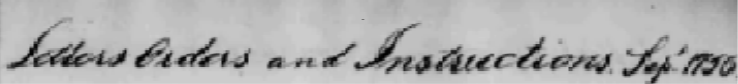
\includegraphics[scale=0.52]{imgs/a_line_img.png} & 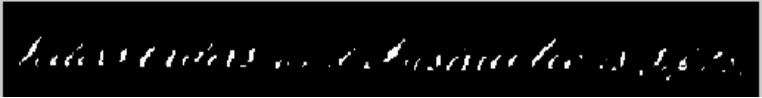
\includegraphics[scale=0.52]{imgs/bloby1x2.png} \\
(a) Ảnh gốc viết tay & (b) Ảnh blob với scale $\sigma_y = 1, \sigma_x = 2$ \\\\

\includegraphics[scale=0.52]{imgs/bloby2x4.png} & 
\includegraphics[scale=0.52]{imgs/bloby4x16.png} \\
(c) Ảnh blob với scale $\sigma_y = 2, \sigma_x = 4$ & (d) Ảnh blob với scale $\sigma_y = 4, \sigma_x = 16$\\\\

\includegraphics[scale=0.52]{imgs/bloby6x36.png}\\
(e) Ảnh blob với scale $\sigma_y = 6, \sigma_x = 36$
\end{tabular}
\label{tab:gt}
\captionof{figure}{Ảnh dòng chữ viết tay và đầu ra với các tỷ lệ khác nhau}
\end{table}
%end ảnh 2

Thuật toán trong bài báo này cần chọn ra $\sigma_y$ và hệ số nhân $\eta $ để trích xuất blob. Giá trị cực đại của phạm vi không gian của các blob chính là trường hợp lý tưởng nhất để tiến hành lọc, đây là phân tích giúp ta đưa ra được phương pháp chọn tỷ lệ đơn giản nhất. Để đo được độ thay đổi giữa phạm vi không gian của các blob so với tỷ lệ ta định nghĩa $\zeta_i$ đại diện cho khoảng rộng của blob thứ i. Như vậy tổng khoảng rộng của bộ blob A (tức một dòng) sẽ là $A = \sum_{i = 1}^{n} \zeta_i$.\par

\textbf{Lựa chọn $\eta$}. Tham số $\sigma_y$ và $\sigma_x$ sẽ có nhiệm vụ tìm được kích thước không gian của một từ. Một đặc tính quan trọng của một từ là tỷ lệ khung hình. Phân tích thủ công trên và bức ảnh cho thấy tỷ lệ khung hình trung bình của một văn bản dạng ảnh nằm trong khoảng $3.0 - 5.0$. Trước đó chúng ta đã định nghĩa hệ số nhân $\eta$ là $\sigma_x / \sigma_y$. Một phân tích khác trên vài bức ảnh khi để $\sigma_y$ là một hằng số ($\sigma_y$ không đổi) cho thấy cực trị của khoảng rộng khi áp dụng $\eta$ này nằm trong khoảng $3 - 5$. Ảnh một dòng chữ và phác đồ phân tích của ảnh được biểu diễn ở hình 3. Trong hình này, cực trị đạt được trong vùng 3.5 đến 4. Phân tích này cùng với quan sát cho thấy tỷ lệ khung hình trung bình của một từ nằm trong khoảng $3.0 - 5.0$ cho phép chúng ta chọn $\eta$ nằm trong khoảng này. Để phục vụ cho các phân tích tiếp theo thì ta chọn cụ thể là $\eta = 4$.

%ảnh 3
\begin{table}[ht]
\centering
\begin{tabular}{cL}
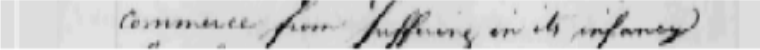
\includegraphics[scale=0.52]{imgs/a_line_img_1.png} & 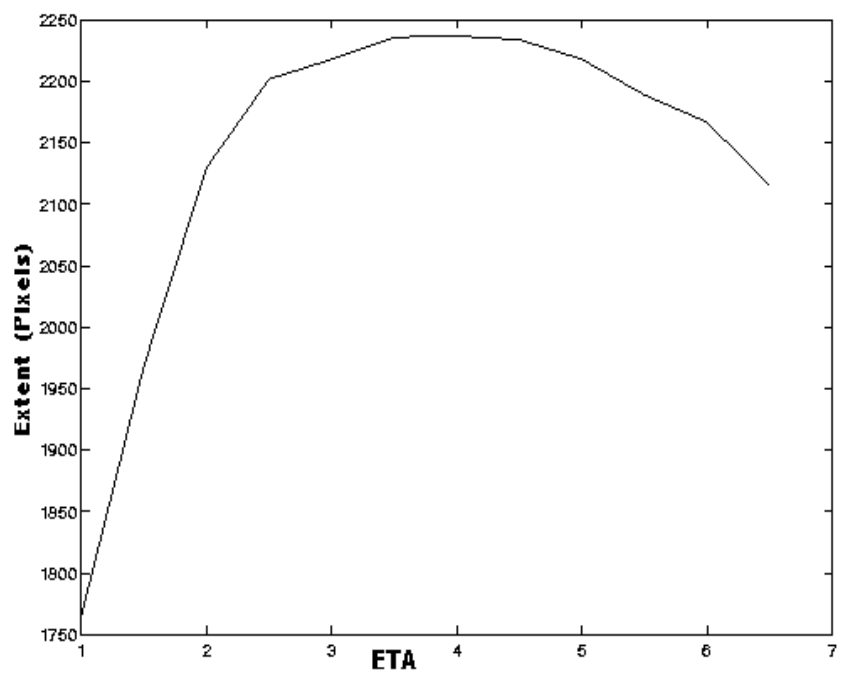
\includegraphics[scale=0.52]{imgs/ploty2n38.png} \\
(a) Ảnh gốc viết tay & (b) Đồ thị tương quan giữa khoảng rộng và $\eta$, trên ảnh này thì $\sigma_y = 2$, đạt cực trị khi $\sigma_y = 3.8$ \\
\end{tabular}
\label{tab:gt}
\captionof{figure}{Độ biến thiên của khoảng rộng blob và $\eta$ với $\sigma_y$ không đổi}
\end{table}
%end ảnh 3

\textbf{Lựa chọn $\sigma_y$}. Như trong hình 4, tổng khoảng rộng có cực trị thay đổi khi $\sigma_y$ thay đổi nhưng $\eta$ không đổi. Hình 4 cũng cho ta thấy cực trị đã bị dịch chuyển ra sao khi kích thước (cụ thể là chiều cao) của các ký tự thay đổi. Khi đưa vào thực nghiệm, ta phát hiện ra $\sigma_y$ là một hàm của chiều cao của các từ (điều này cũng cho thấy sự liên quan với chiều quan của cả dòng chữ). Ước lượng giá trị của $\sigma_y$ có thể suy ra được bằng cách dùng chiều cao của dòng chữ như sau.

\begin{equation}
\sigma_y = k \times \text{Chiều cao của dòng chữ}
\end{equation}

với $0 < k < 1$. Các giá trị tỷ lệ lân cận sau đó sẽ được kiểm chứng để xác định giá trị cực đại. Trong giai đoạn triển khai tác giả đã sử dụng $k = 0.1$ và thử nghiệm với $\sigma_y = 0.3$. Hai giá trị này đã được xác định khi thực nghiệm và cho ra kết quả khá tốt trên nhiều tập dữ liệu ảnh khác nhau.

%ảnh 4
\begin{table}
\centering
\begin{tabular}{LL}
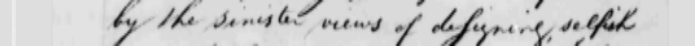
\includegraphics[scale=0.52]{imgs/a_line_img_smaller_height.png} & 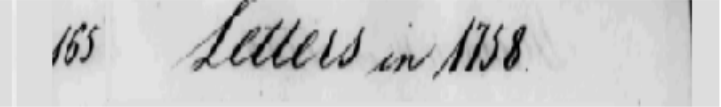
\includegraphics[scale=0.52]{imgs/a_line_img_larger_height.png} \\
(a) Ảnh gốc viết tay với chiều cao thấp & (b) Ảnh gốc viết tay với chiều cao cao hơn \\
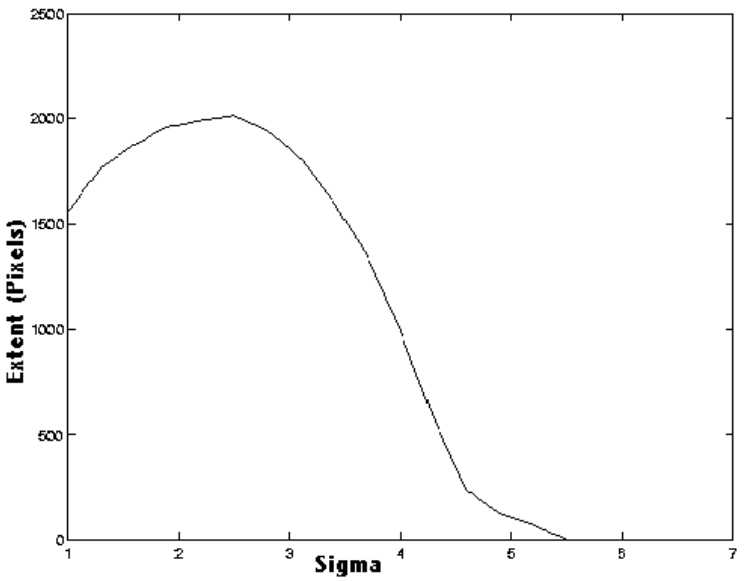
\includegraphics[scale=0.52]{imgs/ploty25n4.png} & 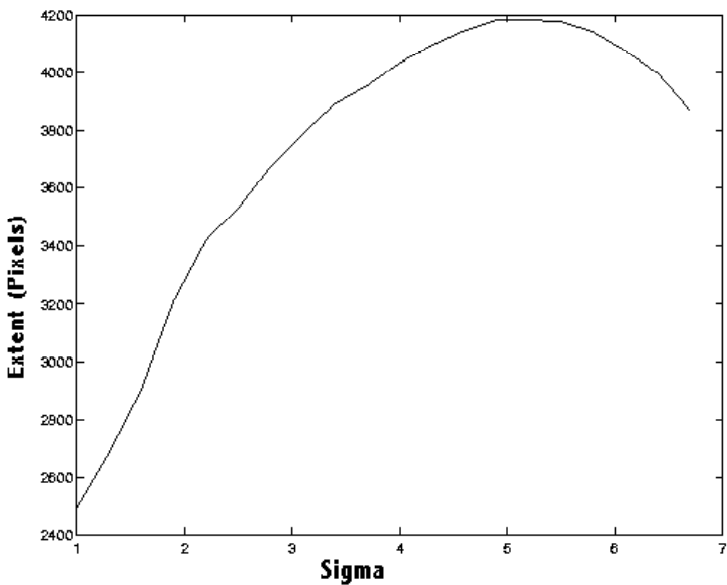
\includegraphics[scale=0.52]{imgs/ploty6n4.png}\\
(c) Đồ thị tương quan giữa khoảng rộng và $\sigma_y$, cực trị đạt được khi $\sigma_y = 2.5$ & (d) Đồ thị tương quan giữa khoảng rộng và $\sigma_y$, cực trị đạt được khi $\sigma_y = 6.0$
\end{tabular}
\label{tab:gt}
\captionof{figure}{Độ biến thiên của khoảng rộng blob và $\sigma_y$ với $\eta = 4$ không đổi.}
\end{table}
%end ảnh 4

\section{Trích xuất blob và hậu xử lý} %2.6
\label{sec:2.6}
Các blob sau đó sẽ được ánh xạ lại với ảnh gốc để xác định vị trí các từ. Một cách làm phổ biến chính là ghim blob vào một khu vực giới hạn (gọi là bounding box) được xác định thông qua phân tích các thành phần liên thông. Việc định vị khi biểu diễn từ bằng blob không được đảm bảo. Đồng thời một phần của các từ, đặc biệt là phần nhô lên và nhô xuống của chữ cái, sẽ bị lỗi do công đoạn tách dòng và làm mịn (làm mờ) ảnh trước đó. Vì lý do trên, bounding box sẽ được mở rộng để bao được hết phần nhô lên và nhô xuống đó. Đến giai đoạn này một bộ lọc bề mặt sẽ được sử dụng để loại bỏ đi các cấu trúc nhỏ do nhiễu ảnh.

\end{document}
